\documentclass[11pt]{article}
  \usepackage{fullpage}
  \usepackage{amsmath, amsfonts}
  \usepackage{etoolbox}
  \usepackage{algorithmicx}
  \usepackage{graphicx}
  
  
  
  \title{CS4780/5780 Homework 1}
  \author{Due: Thursday 09/13/2018 11:55pm on Gradescope}
  \date{}
  \begin{document}
    \maketitle
    \noindent
    \textbf{Note: For homework, you can work in a team of 5. Please include your teammates' NetIDs and names on the front page and form a group on Gradescope. (Please answer all questions within each paragraph.)}
    \section*{Problem 1: Train/Test Splits}
    \begin{enumerate}
      \item Suppose your boss Robin asks you to develop a machine learning system that can classify images into object categories. The dataset consists of 100,000 real images with the following properties:
      \begin{itemize}
        \item Each image consists of only one object and is associated with exactly one category. 
        \item There are 20 categories.
        \item There are 5,000 images per category.
        \item In real life (after deployment) all categories are equally likely to appear. 
      \end{itemize}
      Using your knowledge from CS4780, please frame this task as a supervised learning problem. Describe your setup formally and explain how you would split the data into train/validation/test. 
       
      \item Once deployed, a dissatisfied customer (Kilian) points out that five of the categories have a disproportionally high classification error rate. As he is a very nice guy he offers you additional 10,000 images for each one of these five categories, to be added to the original data set and for you to re-train your system. What would go wrong if you simply add these additional images to the original data set and proceed as described in the previous question? What changes would you suggest should be made to the new setup?
    \end{enumerate}
    
  \section*{Problem 2: K-nearest Neighbors}
  \begin{enumerate}
    \item Consider you have the following 2D dataset (with binary class labels) as shown in Figure 1:
    \begin{itemize}
      \item Class $+1$: $\{(1, 2), (1, 4), (5,4)\}$
      \item Class $-1$: $\{(3, 1), (3, 2)\}$
    \end{itemize}
	\begin{figure}[h!]
		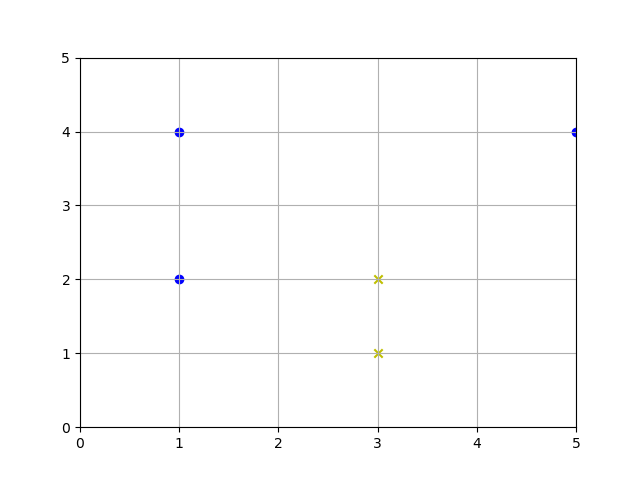
\includegraphics[width=8cm]{Graph1.png}
		\centering
		\caption{Data points in Problem 2.1. Blue = +1, Yellow = -1}
	\end{figure}
    Suppose the data is strictly confined within the $[0, 5] \times [0, 5]$ grid. Draw the decision boundary for a 1-NN classifier with Euclidean distance.  How would the point $(5,1)$ be classified?
    \item Your Finnish friend Aleksandra works with the same data set, however she measured the first coordinate in centimeters instead of meters (the second dimension is unchanged). The data thus becomes:
    \begin{itemize}
      \item Class +1: $\{(100, 2), (100, 4), (500,4)\}$
      \item Class -1: $\{(300, 1), (300, 2)\}$
    \end{itemize}
	Does her 1-NN classifier classify points differently? What will she predict for the original test point $(5,1)$, which she represents as $(500,1)$?
    

    \item $k$-NN can also be used for regression (\emph{i.e.} your labels are real values now). Here, instead of predicting the most common label amongst the neighbors, we predict the label average. Suppose you have the following dataset: 
    \begin{center}
      \begin{tabular}{|c|c|}
        \hline
        $\mathcal{X}$ & $\mathcal{Y}$ \\
        \hline
        (0,0) & 1.0 \\
        (1,1) & 2.5 \\
        (2,3) & 3.0 \\
        (3,1) & 1.0 \\
        (2,1) & 2.5 \\
        \hline
      \end{tabular}
    \end{center}
    where $\mathcal{X}$ is the feature vector and $\mathcal{Y}$ is the label. What would be the label for $(0,1)$ if we use 2-NN with Euclidean distance?
    \item In real life it can happen that a test point has some features missing (e.g. because a sensor dropped, or a measurement couldn't be made). Can we still use K-NN in these cases? If yes, explain how.   
    \item Does it take more time to train a $k$-NN classifier or to apply a $k$-NN classifier? Explain your reasoning. Please assume that the data is on the magnitude of millions of points.
    \item $k$-NN classifiers are known to suffer from the curse of dimensionality. However, in class we showed that $k$-NN actually works on images, which are often high dimensional. Explain why.
  \end{enumerate}

   \section*{Problem 3: Curse of Dimensionality}
   \begin{enumerate}
	\item Remember that the volume of a d-dimensional with radius $r$ can be computed as:
	\begin{equation}
		V_d(r)=\frac{\pi^{\frac{d}{2}}}{\Gamma(\frac{d}{2}+1)} r^{d},
	\end{equation}
	where $\Gamma()$ is a function independent of $r$ and can be treated as a constant. 	 
	\begin{enumerate}
		\item Consider a sphere in $d=3$ with radius $r$. Compute what fraction of the volume remains if we decreases the radius by just $1\%$, i.e. compute $\frac{V_3(0.99r)}{V_3(r)}$. 
	\item Compute the same ratio in $d=10,000$ (a typical dimension for a machine learning data set). 
	\end{enumerate}
	What do you conclude about the volume around the surface and inside the interior of high dimensional spheres? (Optional: Close your eyes and try to visualize a sphere in $d=10,000$. Discuss as a group what it could look like. )
   \end{enumerate}

\end{document}
    
